%! TEX root = ../../main.tex

\subsection{Automating a Microservice's Deployment}%
\label{sub:Automatic_a_Microservices_Deployment}
So far this thesis already introduced the concept of microservices and how they
can be deployed using a container orchestration solution; in this case
Kubernetes. Yet the deployment options offered in chapter~\ref{sub:Kubernetes}
all have to executed by hand. Additionally chapter~\ref{sub:Kubernetes}
presupposes that the container's image is already available on a central image
repository. The basic Docker development workflow in
figure~\ref{fig:docker_workflow} also assumes that developers manually builds
the service's image on their local machine and push them to the central
repository. While this is still a valid possibility, the process consumes a lot
of extra time spent by the developer and is error prone. Furthermore, in such a
manual process no central quality control can force policies upon the source
code of each service. These problems can be solved by introducing an additional
automation component: A \ac{CI} and \ac{CD} server. This section will outline
the basic principles of such a server and apply them to an exemplary \ac{SaaS}
solution \textit{Microsoft DevOps}.

\subsubsection{Continuous Integration}%
\label{ssub:Continuous_Integration}
The basis for continuously releasing a software, in this case a microservice,
is a \ac{CI} concept. This concept spans a wide range of topics including the
\begin{itemize}
  \item compilation of source code,
  \item integration of databases,
  \item execution of tests,
  \item application of rules upon the source code using inspection and
  \item preparation of documentation and feedback of each build \autocite[pp.
    12-20]{MatyasContinuousIntegration2007}.
\end{itemize}

\autocite{MatyasContinuousIntegration2007} also includes the continuous
deployment of software though this will be covered separately in
chapter~\ref{ssub:Continuous_Deployment}. Each iteration of the steps listed
above is called a \textit{build}. A build assembles the source code and makes
sure that the software works as intended \autocite[p.
4]{MatyasContinuousIntegration2007}. The \textit{integration} of software
usually consists of the steps portrayed in
figure~\ref{fig:ci_pipeline_classic}.

\begin{figure}[H]
\begin{center}
  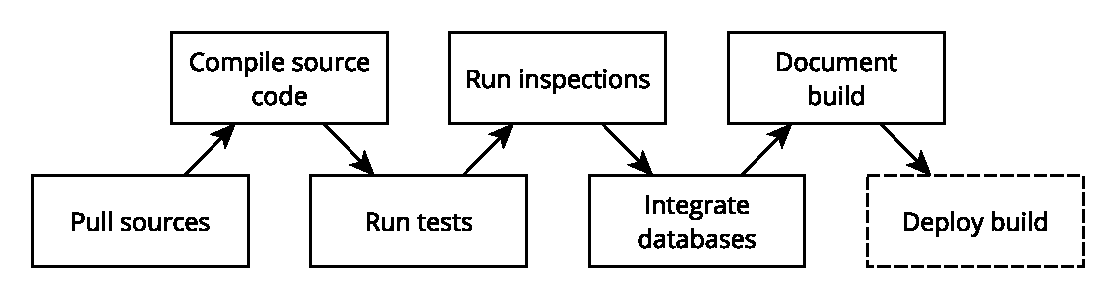
\includegraphics[scale=0.7]{images/figures/ci_classic.pdf}
\end{center}
\caption[The most common, abstracted \ac{CI} pipeline for a classic
software.]{The most common, abstracted \ac{CI} pipeline for a classic
software (adapted from \autocite[Fig. 1-4]{MatyasContinuousIntegration2007}).}%
\label{fig:ci_pipeline_classic}
\end{figure}

In order for this pipeline to be implemented, a number of prerequisites exist.
First, the project's source code has to be tracked in a \ac{VCS}. The \ac{VCS}
holds the source code in a central place that can be accessed by all developers
\autocite[Ch.  1]{MatyasContinuousIntegration2007}. In addition, the \ac{VCS}
allows multiple developers to work on different tasks for the same project
concurrently. The \ac{VCS} acts as the data foundation for the integration
process.

\begin{figure}[H]
\begin{center}
  \missingfigure{Add figure that shows a linear proceeding of all CI steps.}
\end{center}
\caption{The \ac{CI} pipeline in a containerized project.}%
\todo{Add description of the term pipeline.}
\label{fig:containerCIWorkflow}
\end{figure}

\todo{Add Docker mutli stage build process description.}

Furthermore, the code produced by the developers has to be checked in the
\ac{VCS} regularly. Only then may the \ac{CI} process detect problems early and
inform the responsible developer of the breaking change. Code should be checked
in more then a couple of times a day \autocite[p.
59]{JezHumbleContinuousDelivery2010}.
% TODO: Maybe add statement that states that CI is not compatible with
% branching - Maybe refute?

A requirement for successful continuous integration is an extensive test suite.
When building software, a successful build does not necessarily imply that the
software works as indented. E.g.\ a calculator service might compile but as
long as the addition function returns \texttt{1 + 1 = 3}, the code should not be
classified as performing correctly. The test suites must also be able to be
executed automatically \autocite[p. 60]{JezHumbleContinuousDelivery2010}.

\autocite[p. 62]{JezHumbleContinuousDelivery2010} further states that the
developers should be able to build and test the software in any environment
under their control; including their local machine. This is particularly well
feasible when working with microservices that will eventually be deployed to a
Kubernetes cluster. Kubernetes is not only able to run in a datacenter but also
on a developer's machine.

As long as all these requirements are fulfilled, a \ac{CI} process can be
successfully used. Though when applying \ac{CI} to microservice architectures,
an additional remarks needs to be made. The traditional \ac{CI} process does
not specify how the software should be build \autocite[p.
18]{MatyasContinuousIntegration2007}. In a monolithic project, a usual outcome
of the \ac{CI} process is a bundle of the built software that also includes all
database schemas and installation scripts. This piece of data is also referred
to as an \textit{artefact}. As outlined in
chapter~\ref{ssub:Dockerizing_a_Microservice}, microservices are shipped as
Docker images. Thus a successful build process always has to produce a Docker
image and push it to a central image repository. The \ac{CI} artefact in a
microservice project hence would be a runnable Docker image. That Docker image
bundles the full runtime environment and thus does not need to include the
installation instructions and scripts.

\subsubsection{Continuous Deployment}%
\label{ssub:Continuous_Deployment}
Now that the \ac{CI} process has produced a runnable artefact, the next step is
to deploy this artefact to an environment. The environment to which the
artefact is deployed can be freely chosen. However the most typical
environments a software lives in are outlined in the upcoming
chapter~\ref{sub:Deployment_Environments}. In general \ac{CD} is a set of
methods and steps that deploys software scheduled to an end user. A software
that is not successfully deployed does not exist. \ac{CD} helps developers to
overcome this problem by giving them a framework for automating this process.
\autocite[pp.  190]{MatyasContinuousIntegration2007}.

The need for automating the deployment process becomes clear when taking a look
at Amazon. Amazon deploys its software approx.\ every 11.6 seconds. This
statistic only includes deployments to production and does not cover Amazon's
other deployment environments like development
\autocite{JenkinsVelocityCulture2011}. When encompassing this sheer amount of
releases and such short release cycles it becomes clear that a deployments have
to be automated.

To successfully implement \ac{CD} a number of requirements have to be
fulfilled: \todo[color=green!50]{Such a list should also be added to the CI section for future reference.}
\begin{itemize}
  \item Labels have to be applied to the files inside the \ac{VCS}
    \autocite[pp. 191-194]{MatyasContinuousIntegration2007}.
  \item Labels have to be applied to each build \autocite[pp.
    195f.]{MatyasContinuousIntegration2007}.
  \item The environment to which the software will be deployed has to be
    \textit{clean} \autocite[pp. 194f.]{MatyasContinuousIntegration2007}.
  \item All tests must pass in order for a software to be declared working
    \autocite[p. 196]{MatyasContinuousIntegration2007}.
  \item A feedback report has to be created at the end of each build
    \autocite[pp. 196-198]{MatyasContinuousIntegration2007}.
  \item Releases must be able to be rolled back \autocite[p.
    199]{MatyasContinuousIntegration2007}.
\end{itemize}

Labels should be applied to both files stored inside the \ac{VCS} as well as
the outcome of each build. Files with the same label can be considered to be a
group. Further in the worst case, labels allow software to be rolled back
easily without having to track the files of a release individually. A new
release from the same files can be created with ease when all files are tracked
with a label \autocite[pp. 191-194]{MatyasContinuousIntegration2007}.

Build labels on the other hand do not track uncompiled files. They are applied
to the artefacts of a build and are unique. Hence, a build artefact produced
from a snapshot of files e.g.\ labelled \texttt{release\textunderscore 2.0.1}
could be labelled \texttt{release\textunderscore 2.0.1-\textbf{1}}. Each time
the artefact is rebuilt, the last number at the end of the label (\texttt{1})
is incremented. When using a labelled build the features, defects and
requirements can be traced to a specific a specific release version. Without
labels it would not be possible to e.g.\ pin issues to an explicit release
\autocite[pp. 195f.]{MatyasContinuousIntegration2007}.

In addition, a \textit{clean} environment has to be provided for each
deployment. That means that no leftover files from other deployment are still
present on a machine when the next deployment is applied. Any leftover files
may distort the execution of the software and thus may mask or provoke unwanted
behaviour. \autocite{ArtacDevOpsIntroducingInfrastructure2017} offers a
layer-based approach to avert this problem. In this approach a \textit{machine}
is composed of multiple \textit{layers}. Each layer is stacked on top of the
previous one and together they build the environment in which the application
is executed. The layers range from the \ac{OS}, its configuration files, any
middleware components (like an application server) or additional pieces of
software (like a database server) up to the actual software. Each time a new
deployment is applied, the complete stack is purged and rebuilt from the ground
up \autocite[p. 194]{MatyasContinuousIntegration2007}.

In a monolithic architecture this approach might suffice. It, however, has to
be adapted to also support a containerized microservice architecture. First of
all, each time a container for a microservice is created, only a few layers on
top of the stack are rebuilt. When e.g.\ deploying an application that depends
on a \textit{NGINX} web server, the web server and any underlying layers can
be reused as part of a Docker base image. So only the layers on top of the web
server have to be reapplied. This process also ensures that the environment to
which the software is deployed is clean while being more efficient
than rebuilding each layer. In addition, the use of a container orchestration
solution like Kubernetes has the advantage of defining the underlying
infrastructure as code. \ac{IasC} allows the infrastructure to be defined
inside a \enquote{single commonly available source of truth}, most frequently
stored inside a \ac{VCS}, without the need for additional administrators
\autocite{ArtacDevOpsIntroducingInfrastructure2017}. In Kubernetes,
infrastructure changes can be performed by applying these configuration files.
When realized correctly, the developer performing these changes does not have
to worry about past infrastructure configurations remaining in the system.
Kubernetes keeps track of old resources and manages them accordingly
\autocite{AuthorsDeployments2019}. The \ac{IasC} paradigm further supports the
aim of always producing a clean deployment environment.

It is a common approach to run tests locally before pushing code changes to the
\ac{VCS}. The local environment however most often differs, even if only in
minor details, from the actual environment the application will be deployed in.
Hence it can not be guaranteed that a passing test on the local machine also
produces the same result in the deployment environment. This is the reason why
\textit{all} tests also have to be completed in the deployment environment. The
tests do not only have to be executed, all tests need to pass. Only then it can
be guaranteed that the software is working as expected \autocite[p.
196]{MatyasContinuousIntegration2007}. As already shown in
figure~\ref{fig:containerCIWorkflow} the container is build in multiple stages.
The tests can be executed a second time in an early build stage. The build then
only proceeds if all tests pass a second time inside that early build stage.

\begin{figure}[H]
\begin{center}
  \missingfigure{Add extended CI container build process figure that shows the
  additional test stage inserted in the multi stage process.}
\end{center}
\caption{Re-execution of the tests during the Docker build process in a
containerized project.}%
\label{fig:containerCIWorkflowExtended}
\end{figure}

Regardless of the outcome of the build, a feedback report should be generated.
That report includes information about the changed files, new features and
fixes. Any interested team member can then verify that the build contains the
desired aspects \autocite[pp. 196-198]{MatyasContinuousIntegration2007}.

Lastly the \textit{Cloudflare} outage in July 2019 showed the importance of
having a working process in place to roll back any release. Even though
Cloudflare had a rollback plan in place, they could not successfully execute
it. This resulted in a unavailability of Cloudflare's global network for 27
minutes \autocite{Graham-CummingDetailsCloudflareoutage2019}. The existence of
a working and fast rollback process allows defects introduced by a release to
be temporarily resolved by simply rolling back to the previous version
\autocite[p. 199]{MatyasContinuousIntegration2007}.

Given that these requirements are fulfilled, it is ensured that the automated
build produces a working software that can be released at any time \autocite[p.
200]{MatyasContinuousIntegration2007}.

